\documentclass[t,compress,aspectratio=169]{beamer}
\usetheme{neutral}

\usepackage[english]{babel}
\usepackage[utf8]{inputenc}
% \usepackage[lighttheme]{uobham-beamer}
\usepackage{listings}
\usepackage[UKenglish]{datetime}
\usepackage{algpseudocode}
\usepackage{fontawesome5}
\usepackage{listings}
\usepackage{multirow}
\usepackage{booktabs}
\usepackage{soul}
\usepackage{minted}
\newcommand{\vehicle}[1]{{\mintinline{haskell}{#1}}}

\usepackage{ulem}
\newdateformat{UKvardate}{%
	\monthname[\THEMONTH] \THEDAY \ \THEYEAR}

% Set to 1 or comment to disable transparency and enable full opacity.
\setblockbodyopacity{0.8}

% Listings
\definecolor{cident}{rgb}{1,0.33,0.42}
\definecolor{ckeyw}{rgb}{1,0.2,0.8}
\definecolor{ccomm}{rgb}{0,0.8,0}
\definecolor{cstr}{rgb}{0.8,0,0}

\lstset{language=[LaTeX]{TeX},
  basicstyle=\footnotesize\ttfamily,
  keywordstyle=\color{ckeyw}\bfseries,
  identifierstyle=\color{cident}\bfseries,
  commentstyle=\color{ccomm},
  stringstyle=\color{cstr},
  showstringspaces=false,
  breaklines=true,
  breakatwhitespace=true,
  tabsize=2,
%   numbers=left,
%   stepnumber=1,
%   firstnumber=1,
%   numberfirstline=true,
  }

\usepackage{stmaryrd}
\usepackage{local-macros}
\newcommand{\distance}[2]{|#1 - #2|}
\newcommand{\outputdistance}[2]{||#1 - #2||}
%\newcommand{\x}{\vect{x}} 		% Arbitrary input
%\newcommand{\xt}{\hat{\x}} 		% Training input
\newcommand{\xs}{\x} 			% Sampled input
\newcommand{\xp}{\tilde{\x}} 	% Perturbed input

%\newcommand{\y}{\vect{y}} 		% Arbitrary output
\newcommand{\yt}{\hat{\y}} 		% Training output
\newcommand{\ys}{\y} 			% Sampled output



\newcommand{\SR}[2]{SR(#1, #2)} % Standard robustness
\newcommand{\LR}[2]{LR(#1, #2)} % Lipschitz robustness
\newcommand{\CR}[1]{CR(#1)} % Classification robustness
\newcommand{\SCR}[2]{SCR(#1,#2)} % Approximate class. robustness
\usepackage{pifont}
\definecolor{forestgreen}{RGB}{35, 142, 35}
\definecolor{lightaisecred}{RGB}{237, 41, 57}
\newcommand{\yes}{\textcolor{forestgreen}{\ding{51}}}
\newcommand{\no}{\textcolor{aisecred}{\ding{55}}}
\newcommand{\good}[1]{\textcolor{forestgreen}{#1}}
\newcommand{\average}[1]{\textcolor{orange}{#1}}
\newcommand{\bad}[1]{\textcolor{aisecred}{#1}}

\newcommand{\wrapp}[2]{\begin{minipage}[t]{#1\columnwidth}
    \centering #2
\end{minipage}}


\usepackage{amsfonts,amsmath,amssymb,amsthm}
\usepackage[all]{xy}
\usepackage{array,url}
\usepackage{textcomp,textgreek}
\usepackage{pgfplots}
\usepackage{float}
\pgfplotsset{width=5cm,compat=1.9}
\usepackage{mdframed,wrapfig,subcaption}
%\usepackage[font=footnotesize,labelfont=it
%\usepackage[latin1]{inputenc}
\usepackage{babel}
\usepackage{color}
%\usepackage{url}
\usepackage{hyperref}
\usepackage{fancyvrb}
%\usepackage{tikz}
\usepackage{alltt}
%\usepackage{etex, xy}
%\usepackage{cibeamer}
\usepackage{tikz}
\usetikzlibrary{arrows,shapes}
%\xyoption{all}
%\usepackage{listings}
%\input macro
\usepackage{cancel, comment}
\usepackage{verbatim}
\usepackage{slashbox}
\usepackage{ulem}

\newcommand{\tikzmark}[1]{\tikz[remember picture] \node[coordinate] (#1) {#1};}
\newcommand{\semitransp}[2][35]{\color{fg!#1}#2}

\usepackage[absolute,overlay]{textpos}
\beamertemplatenavigationsymbolsempty
\usepackage{ijcnn-diagram}

\usepackage[all]{foreign}

\newcommand{\fstar}{F$^\ast$\xspace}
\newcommand{\starchild}{StarChild\xspace}
\newcommand{\lazuli}{Lazuli\xspace}
\newcommand{\sapphire}{Sapphire\xspace}
\newcommand{\cL}{{\cal L}}
%\newcommand{\Real}{{\mathbb R}}
\usepackage{makecell}
\DeclareMathOperator{\linear}{linear}
\DeclareMathOperator{\relu}{relu}
\DeclareMathOperator{\sigmoid}{sigmoid}
\DeclareMathOperator{\softmax}{softmax}
\DeclareMathOperator{\neuron}{neuron}
\DeclareMathOperator{\truthy}{truthy}
\DeclareMathOperator{\falsey}{falsey}
\DeclareMathOperator{\neurontest}{test}
\usepackage{ellipsis}
\renewcommand{\ellipsisgap}{-0.25em}

\definecolor{beamer@headercolor}{RGB}{204, 72, 71}
\colorlet{beamer@barcolor}{beamer@headercolor!70!black}

\definecolor{beamer@progresscolor}{HTML}{ffe960}
%\setbeamercolor{AAUsimple}{fg=aisecred!20,bg=aisecred}
%\setbeamercolor{sidebar}{bg=aisecred!20}
% Change the color of the structural elements:
%\setbeamercolor{structure}{fg=aisecred}
% Change the frame title text color:
\setbeamercolor{frametitle}{fg=aisecpurple!20!black}
\setbeamercolor{definition}{fg=aisecaisecred!10!white}


% Change the normal text color background:
\setbeamercolor{normal text}{fg=black,bg=gray!10}
\setbeamercolor{subtitle}{fg=white!90!aisecpurple,bg=gray!10}

\usepackage{soul}
\makeatletter
\let\HL\hl
\renewcommand\hl{%
  \let\set@color\beamerorig@set@color
  \let\reset@color\beamerorig@reset@color
  \HL}
\makeatother

%\usetikzlibrary{decorations.pathreplacing,shapes.arrows}
\newcommand\BackgroundPicture[1]{%
  \setbeamertemplate{background}{%
   \parbox[c][\paperheight]{\paperwidth}{%
      \vfill \hfill
\includegraphics[width=1\paperwidth,height=1\paperheight]{#1}
        \hfill \vfill
     }}}
\usepackage{xcolor,colortbl}
%\usepackage{listings}
\definecolor{Gray}{gray}{0.85}

\newcommand{\question}[1]{\begin{description}
		\item[\textbf{Question.}] #1
\end{description}}

\newcommand{\task}[1]{\begin{description}
		\item[{\textcolor{aisecred}{\textbf{Task.}}}] #1
\end{description}}

\newcommand{\focus}[1]{\begin{description}
		\item[{\textcolor{aisecred}{\textbf{Note.}}}] #1
\end{description}}


\def\checkmark{\tikz\fill[scale=0.4,color=green](0,.35) -- (.25,0) -- (1,.7) -- (.25,.15) -- cycle;}
\newcommand{\down}[1][aisecred]{{\color{#1}\scalebox{1.4}[.7]{\,$\blacktriangledown$\,}}}
\newcommand{\up}[1][green!70!black]{{\color{#1}\raisebox{0.1em}{\scalebox{1.4}[.7]{\,$\blacktriangle$\,}}}}
\newcommand{\stall}[1][yellow!70!aisecred]{{\color{#1}\raisebox{0.1em}{\scalebox{1.4}[.5]{\,$\blacksquare$\,}}}}

\title{Neural Network Verification With Vehicle: Chapter 3 - Robustness}

\subtitle{VeTSS Summer School'23}  % could also be a conference name

\date{\today}

\author{Luca Arnaboldi\inst{1}  \and Ekaterina Komendantskaya\inst{2} \and Matthew Daggitt (online) \inst{3}}

% - Give the names in the same order as they appear in the paper.
% - Use the \inst{?} command only if the authors have different
%   affiliation. See the beamer manual for an example



\institute{$^{1}$University of Birmingham $\cdot$ $^{2}$University of Southampton $\cdot$ $^{3}$Heriot-Watt University}

\setbackgroundgraphics{img/surrey}
\setbackgroundgraphicscopy{image by \copyright {\bf University of Surrey}}
% \setlogographics{img/artwork-logo}
% \settitlegraphics{img/cloud}

\setcirclelogographics{img/artwork-logo-circle}

% specify a logo on the titlepage (you can specify additional logos an include them in
% institute command below
% \pgfdeclareimage[height=2cm]{titlepagelogo}{\logographics} % placed at the title page
% % \pgfdeclareimage[height=7cm]{titlepagelogo2}{\titlegraphics} % placed on the title page


% \titlegraphic{% is placed at the bottom of the title page
%   \pgfuseimage{titlepagelogo}
% %   \pgfuseimage{titlepagelogo2}

% %  \hspace{1cm}\pgfuseimage{titlepagelogo2}
% }


\begin{document}
% the titlepage

\setbackground
\begin{frame}[fragile,plain,noframenumbering] % the plain option removes the header from the title page
  \titlepage
\end{frame}
\unsetbackground

\begin{frame}[fragile]{Again - The \st{elephant} ... \st{panda}... gibbon? in the room}

 \centering\includegraphics[width=.9\textwidth]{img/attack.png}
 \vfill
 	\vspace{-2em}

\begin{quote}
		\tiny Goodfellow, I. J., Shlens, J., \& Szegedy, C. (2014). Explaining and harnessing adversarial examples. arXiv preprint arXiv:1412.6572.


	\end{quote}
\end{frame}

% \begin{frame}[fragile]{Some Robustness Issues}

% 	\centering 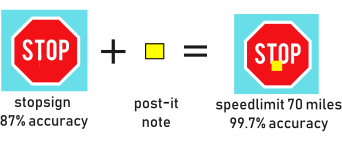
\includegraphics[width=.8\textwidth]{img/fooling-signs.pdf}
% 	\vfill
% 	\vspace{-1em}
% 	\begin{quote}
% 		\tiny Eykholt, K., Evtimov, I., Fernandes, E., Li, B., Rahmati, A., Xiao, C., ... \& Song, D. (2018). Robust physical-world attacks on deep learning visual classification. In Proceedings of the IEEE conference on computer vision and pattern recognition (pp. 1625-1634).

% 	\end{quote}
% \end{frame}

\begin{frame}{This is what a simple Neural Network Property Looks like}

\Large
\begin{block}{Simple NN Property}
Let $f$ be the neural network\\
Let $\hat{x}$ be an input in the training set \\
Let \texttt{$|\cdot - \cdot |$} be some notion of distance\\

Then \[\forall x : | x - \hat{x}| \leq \epsilon \implies | f(x) - f(\hat{x})| \leq \delta\]

\end{block}
% For all input xx, if the distance between xx and the training input x^x^ is less than or equal to ϵϵ, then the distance between the outputs f(x)f(x) and f(x^)f(x^) of the neural network for those inputs is also less than or equal to ϵϵ."

%In simpler terms, the formula is stating that if an input xx is close (within a distance of ϵϵ) to a training input x^x^, then the neural network's predictions for these two inputs xx and x^x^ will also be close (within a distance of ϵϵ) to each other.

\end{frame}

\begin{frame}{In Practice - Robustness of MNIST}

    Let us take as an example the famous MNIST data set by LeCun etal. The images look like this:

    \centering
    \includegraphics[width=0.6\textwidth]{img/MNIST.jpeg}


\end{frame}

%The MNIST dataset, created by Yann LeCun and his colleagues, is a widely used dataset in the field of machine learning and computer vision. It consists of a collection of handwritten digits, each represented as a 28x28 grayscale image. The dataset was initially introduced to serve as a benchmark for evaluating various machine learning algorithms, particularly for image classification tasks. It has played a significant role in the development and testing of new algorithms and techniques in the field.

% Here are some key details about the MNIST dataset:

%     Image Format: Each image in the dataset is a grayscale image of size 28x28 pixels. The pixel values range from 0 to 255, where 0 represents black and 255 represents white. The intensity of the pixels represents the darkness of the corresponding region in the image.

%     Handwritten Digits: The MNIST dataset contains handwritten digits from 0 to 9. Each digit class (0, 1, 2, ..., 9) is represented by a subset of the dataset.

%     Training and Test Sets: The dataset is divided into two main parts: a training set and a test set. The training set contains a large number of labeled examples that are used to train machine learning models. The test set contains a separate set of labeled examples that are used to evaluate the performance of trained models on unseen data.

%     Labeling: Each image in the dataset is associated with a label that indicates the digit it represents. For instance, an image of the digit "7" will have the label 7.

%     Use Cases: The MNIST dataset has been widely used to evaluate the performance of various machine learning algorithms, particularly in the context of image classification and pattern recognition. Researchers often use it to benchmark new techniques and compare their results with established methods.

%     Challenges: While the MNIST dataset has been immensely useful, it's worth noting that it is relatively simple compared to real-world scenarios. The images are well-centered, well-scaled, and the digits are written with a relatively uniform style. As a result, algorithms that perform well on MNIST might not necessarily generalize well to more complex datasets.




\begin{frame}{In Practice - Robustness of MNIST}

   \begin{columns}
        \begin{column}{0.3\textwidth}
            \begin{center}
                        Predicted \textit{\textbf{"0"}} 99\%

             \includegraphics[width=\textwidth]{img/true.png}
             \end{center}
        \end{column}
        \begin{column}{0.3\textwidth}  %%<--- here

            \begin{center}
                        Small perturbation

             \includegraphics[width=\textwidth]{img/eta.png}
             \end{center}
        \end{column}
          \begin{column}{0.32\textwidth}  %%<--- here

            \begin{center}
                        Predicted \textit{\textbf{"5"}} 94\%

             \includegraphics[width=\textwidth]{img/adv.png}
             \end{center}
        \end{column}
    \end{columns}


\end{frame}

\begin{frame}[fragile]{Formal Verification of NN (more details)}
	\vspace{-1em}
	\begin{alertblock}{Definition of Verification for a Black Box Model}
		For a neural network $N : \hat{x} \rightarrow \hat{y}$, the input property $P(\hat{x})$ and the output property $Q(\hat{y})$, does there exist an input $\hat{x_0}$ which satisfies $P(\hat{x_0})$ such that its corresponding output $\hat{y_0}$ satisfies $Q(\hat{y_0})$?
	\end{alertblock}
		\vspace{1em}
	\begin{itemize}

		\item $P(\hat{x})$ characterises inputs checked
		\item $Q(\hat{y})$ characterises the behaviour we \textcolor{aisecred}{DO NOT} wish for
		\item if satisfied, counterexample is returned, else property holds
		%want to ensure that or a given input $\overline{x_i}$ (which represents our image) and given amount of noise $\delta$, classification remains the same
		% x whose distance from x_i is at most delta, according to some distance matrix
		\item the $P$ for robustness is $|\hat{x} - \hat{x_0}|_{ L_{\infty}} \leq \epsilon$ (more on this later)
		\item the $Q$ is, $\bigvee_i(\hat{y}[i_0] \leq \hat{y}[i])$, where $\overline{y}[i_0]$ is the desired label
	\end{itemize}
\end{frame}

\begin{frame}{Or More Simply: Robustness}

\begin{alertblock}{$\epsilon$-ball robustness**}

Formally, we define an $\epsilon$-ball around an image $\hat{\mathbf{x}}$ as:


\begin{itemize}
    \item[] $$\mathbb{B}(\hat{\mathbf{x}}, \epsilon) = \{ \mathbf{x} \in \mathbb{R}^n: |\hat{\mathbf{x}}-\mathbf{x}| \leq \epsilon \}$$
    \item [] where $| ... |$ is a distance function (or $L$-norm) in $\mathbb{R}^n$,
such as Euclidean distance or $L_{\infty}$-norm.
%\item[] so as above $\mathbb{B}%(\hat{\mathbf{x}}, \epsilon)$ :=
%$$\|\hat{x} - \hat{x_0}\| _{ L_{\infty}} \leq \epsilon$$
\end{itemize}
\end{alertblock}
 \vfill
 \footnotesize **There are various types of these
\end{frame}

\begin{frame}{$\epsilon$-ball Visualised}

 \begin{columns}
        \begin{column}{0.35\textwidth}
        \begin{center}
                For every image in the dataset, we assume we can “draw” a small $\epsilon$-ball around it, and guarantee that within that $\epsilon$-ball classification of the network does not change much
        \end{center}

        \end{column}
        \begin{column}{0.6\textwidth}
             \begin{center}
             \vspace{-1em}
    \centering\includegraphics[width=0.45\textwidth]{img/epsballmnist.png}

             \end{center}
        \end{column}
\end{columns}



\end{frame}

\begin{frame}
\vspace {8em}

    \begin{center}
        \Huge{\textcolor{aisecred}{\textbf{How to Specify this in Vehicle?}}}
    \end{center}
\end{frame}




\begin{frame}[fragile]{Formalising $\epsilon$-ball robustness for MNIST networks in Vehicle}

\begin{itemize}
    \item We will see how Vehicle can be used to handle properties that refer directly to the data sets.
    \item  How to specify images (represented as 2D arrays)
    \item User defined parameters in Vehicle
    \item Verification of properties
\end{itemize}
\end{frame}


\begin{frame}{Vehicle Language Overview}{Language Overview}
The Vehicle language contains the following basic types:
\begin{itemize}
\item \vehicle{Bool} - booleans
\begin{itemize}
\item Operations: \vehicle{and}, \vehicle{or}, \vehicle{=>}, \vehicle{not}, \vehicle{if ... then ... else ..., ==, !=}
\end{itemize}
\item \vehicle{Index n} - natural numbers between 0 (inclusive) and n (exclusive).
\begin{itemize}
\item Used for safe indexing into tensors. For example, only the values 0 and 1 have type \vehicle{Index 2}.
\item Operations: \vehicle{==}, \vehicle{!=}, \vehicle{<=}, \vehicle{>=}, \vehicle{<}, \vehicle{>}
\end{itemize}
\item \vehicle{Nat} - natural numbers
\begin{itemize}
\item Operations: \vehicle{==}, \vehicle{!=}, \vehicle{<=}, \vehicle{>=}, \vehicle{<}, \vehicle{>}, \vehicle{+}, \vehicle{*}
\end{itemize}
\item \vehicle{Int} - integer numbers
\begin{itemize}
\item Operations: \vehicle{==}, \vehicle{!=}, \vehicle{<=}, \vehicle{>=}, \vehicle{<}, \vehicle{>}, \vehicle{+}, \vehicle{*}, \vehicle{-}
\end{itemize}
\item \vehicle{Rat} - rational numbers
\begin{itemize}
\item Operations: \vehicle{==}, \vehicle{!=}, \vehicle{<=}, \vehicle{>=}, \vehicle{<}, \vehicle{>}, \vehicle{+}, \vehicle{*}, \vehicle{-}, \vehicle{/}
\end{itemize}
\end{itemize}

\end{frame}

\begin{frame}{Vehicle Language Overview}{Language Overview (continued)}
Next there are two container types:
\begin{itemize}
\item \vehicle{List A} - a list of elements of type \vehicle{A}
\begin{itemize}
\item Used for sequences of data for which one either doesn't care about or don't know the length of.
\item Operations: \vehicle{==}, \vehicle{!=}, \vehicle{map}, \vehicle{fold}
\end{itemize}
\item \vehicle{Tensor A [d1, ..., dn]} - a tensor of elements of type $A$ with dimensions $d1 \times ... \times d_n$.
\begin{itemize}
\item Used for data for which it is important to know the size of. Due to the dependently typed-nature of the language, the dimensions can themselves be arbitrary expressions.
\item Operations: \vehicle{==}, \vehicle{!=}, \vehicle{map}, \vehicle{fold}, \vehicle{!}
\end{itemize}
\end{itemize}
\end{frame}

\begin{frame}[containsverbatim]{Vehicle Language Overview}{Special Mentions: Functions, Networks and Datasets}

\begin{itemize}
    \item The function type is written  \vehicle{A -> B} where \vehicle{A} is the input type and \vehicle{B} is the output type e.g.
    \item[]\begin{minted}{haskell}
add2 : Nat -> Nat
add2 x = x + 2
\end{minted}
\end{itemize}

\begin{itemize}
    \item The language models neural networks as black box functions between tensors
    \item[]\begin{minted}{haskell}
@network
network myNetwork : Tensor Rat [28, 28] -> Tensor Rat [10]
\end{minted}
\end{itemize}

\begin{itemize}
    \item Datasets may be introduced using the \vehicle{dataset} keyword:
\begin{minted}{haskell}
@dataset
dataset myDataset : Tensor Rat [10, 784]
\end{minted}
\end{itemize}



\end{frame}

\begin{frame}[containsverbatim]{Vehicle Language Overview}{Special Mentions: Parameters, Quantifiers and Type Synonyms}

%passed throguh command line
\begin{itemize}
    \item Sometimes the user may not want to hard-code a specific value but rather provide a compile time variable:
    \item[]\begin{minted}{haskell}
@parameter
parameter myParameter : Rat
\end{minted}
\end{itemize}

\begin{itemize}
    \item universal (\vehicle{forall}) and existential (\vehicle{exists}) quantifiers e.g.
\item[]\begin{minted}{haskell}
condition : Bool
condition = forall x . lastOutputPositive x
\end{minted}
\end{itemize}

\begin{itemize}
    \item can declare synonym for types e.g.:
\item[]\begin{minted}{haskell}
type Image = Tensor Rat [28, 28]
@network
network classify : Image -> Tensor Rat [10]
\end{minted}
\end{itemize}



\end{frame}


\begin{frame}[fragile]{Case Study: Initialisation - 2D Arrays and Labels}

Declare input as 2d array (with a label)

\begin{minted}{haskell}
type Image = Tensor Rat [28, 28]

type Label = Index 10
type LabelDistribution = Tensor Rat [10]

\end{minted}


Define what a valid input is (images are within 0 and 1)


\begin{minted}{haskell}
valid : Image -> Bool
valid x = forall i j . 0 <= x ! i ! j <= 1

\end{minted}

\end{frame}

\begin{frame}
\vspace {8em}

    \begin{center}
        \Huge{\textcolor{aisecred}{\textbf{Let's give it a go!}}}
    \end{center}
\end{frame}


% \begin{frame}
% \vspace {8em}

%     \begin{center}
%         \Huge{\textcolor{aisecred}{\textbf{In case it didn't work}}}
%     \end{center}
% \end{frame}

\begin{frame}[fragile]{Case Study: Classifier - Network and Prediction}


The output of the network is a score for each of the digits 0 to 9.

\begin{minted}{haskell}

@network
classifier : Image -> LabelDistribution

\end{minted}



The classifier advises that input image x has label i if the score for label i is greater than the score of any other label j:


\begin{minted}{haskell}

advises : Image -> Label -> Bool
advises x i = forall j .
   j != i => classifier x ! i > classifier x ! j

\end{minted}
\end{frame}


\begin{frame}[fragile]{Case Study: Robustness - User Parameters and Bounds}

define the parameter** epsilon that will represent the radius of the balls that we verify.

\begin{minted}{haskell}

@parameter
epsilon : Rat
\end{minted}

 we define what it means for an image x to be in a ball of size epsilon

\begin{minted}{haskell}

boundedByEpsilon : Image -> Bool
boundedByEpsilon x = forall i j .
    -epsilon <= x ! i ! j <= epsilon

\end{minted}


\footnotesize **N.B \texttt{@parameter }will mean it is specified at runtime

\end{frame}


\begin{frame}[fragile]{Case Study: Robustness - Robust Around a Point}

We now define what it means for the network to be robust around an image x that should be classified as y

\begin{minted}{haskell}

robustAround : Image -> Label -> Bool
robustAround image label = forall pertubation .
  let perturbedImage = image - pertubation in
  boundedByEpsilon pertubation and validImage perturbedImage =>
    advises perturbedImage label

\end{minted}



\end{frame}

\begin{frame}[fragile]{Case Study: Robustness - Robust Image Classification}

Size of input automatically inferaisecred by tool at runtime
\begin{minted}{haskell}

@parameter(infer=True)
n : Nat

\end{minted}

We next declare two dataset (parameter ensures same size)

\begin{minted}{haskell}

@dataset
trainingImages : Vector Image n
@dataset
trainingLabels : Vector Label n
\end{minted}
\end{frame}

\begin{frame}[fragile]{Case Study: Robustness - Robust Image Classification (continued)}

We then say that the network is robust for this data set if it is robust around every pair of input images and output labels.

\begin{minted}{haskell}

@property
robust : Vector Bool n
robust = foreach i .
    robustAround (trainingImages ! i)(trainingLabels ! i)
\end{minted}



\end{frame}

\begin{frame}[fragile]
\frametitle{Full spec $\epsilon$-ball Robustness}
\vspace{-2em}

 \begin{minted}[fontsize=\tiny]{haskell}
type Image = Tensor Rat [28, 28]
type Label = Index 10
@network
classifier : Image -> Vector Rat 10
@parameter
epsilon : Rat

validImage : Image -> Bool
validImage x = forall i j . 0 <= x ! i ! j <= 1

advises : Image -> Label -> Bool
advises x i = forall j . j != i => classifier x ! i > classifier x ! j

boundedByEpsilon : Image -> Bool
boundedByEpsilon x = forall i j . -epsilon <= x ! i ! j <= epsilon

robustAround : Image -> Label -> Bool
robustAround image label = forall pertubation .
let perturbedImage = image - pertubation in boundedByEpsilon pertubation and validImage perturbedImage => advises perturbedImage label

@dataset
trainingImages : Vector Image n
@dataset
trainingLabels : Vector Label n

@property
robust : Vector Bool n
robust = foreach i . robustAround (trainingImages ! i) (trainingLabels ! i)
\end{minted}
\end{frame}



\begin{frame}[fragile]{Case Study: Robustness - Verification}
In order to run Vehicle, we need to provide:

\begin{itemize}
    \item the specification file,
    \item the network in ONNX format,
    \item the data in idx format,
    \item and the dedired $\epsilon$ value.
\end{itemize}





\end{frame}

\begin{frame}[fragile]{Case Study: Robustness - Verification (continued)}
Putting it all together

\begin{minted}{sh}

vehicle verify \
  --specification mnist-robustness.vcl \
  --network classifier:mnist-classifier.onnx \
  --parameter epsilon:0.005 \
  --dataset trainingImages:images.idx \
  --dataset trainingLabels:labels.idx \
  --verifier Marabou

\end{minted}

\end{frame}

\begin{frame}{Concluding Exercise}{PL problems}


\begin{itemize}
\item[$I^O$] Interoperability -- properties are not portable between training/counter-example search/ verification.

\item[$I^{P}$] Interpretability -- code is not easy to understand.

\item[$I^{\int}$] Integration -- properties of networks cannot be linked to larger control system properties.

\item[$E^G$] Embedding gap -- little support for translation between problem space  and input space.
\end{itemize}

\question{Which of these have we addressed in this chapter?}
\end{frame}




\begin{frame}{Conclusions}{What to setup for next session + Excercises!}
	\begin{itemize}
		\item Robustness is currently the most verified property in AI
        \item You should now be familiar with how to specify this and verify networks in Vehicle
        \item Coming Next after the break:
        \begin{enumerate}
            \item \textcolor{aisecred}{Exercise session:} write and verify your own specs (with possibility to extend over the break)

            \begin{itemize}
            \item for writing a spec, install Vehicle: just run

            \texttt{pip install vehicle-lang}

            \item for verifying a spec, you also need Marabou installed

            \texttt{pip install maraboupy}
            \end{itemize}
            \item Property driven training in Vehicle
            \item Integration with Interactive Theorem Provers (Agda)
            \item Practical applications of AI verification
        \end{enumerate}

%		\item Let me know if you want
	\end{itemize}

\vspace{1em}

% \vspace{1em}
% \large \centering Interested? Contact me - \  \  \texttt{\textcolor{aisecred}{\faEnvelope\ l.arnaboldi@bham.ac.uk}}
\end{frame}





\begin{frame}{Exercises}{Easy}


\begin{block}{Robustness (for those familiar with the problem)}
\footnotesize{
\begin{itemize}
\item Run and try a variety of $\epsilon$-values
The spec and network can be found at:
\url{https://github.com/vehicle-lang/tutorial}:\\
\url{exercises/Chapter 2. Getting Started/mnist-robustness}

\item Using the given neworks and data, verify robustness via Vehicle.
\item \textcolor{aisecred}{Exercises 3.5.1, 3.5.2 and 3.5.3}
\end{itemize}}
\end{block}

\begin{alertblock}{Robustness (for those NOT familiar with the problem)}
\footnotesize{Study the chapter ``Proving Neural Network Robustness" here: \url{https://vehicle-lang.github.io/tutorial/}}
\end{alertblock}
\end{frame}

\begin{frame}{Exercises}{More Advanced}

\begin{block}{More Robustness properties in the same spec}

\begin{itemize}
\item Fill in missing code in the Robustness spec available at
\url{https://github.com/vehicle-lang/tutorial}, at \\
\url{examples/Chapter 3. Robustness/}
 \item \textcolor{aisecred}{Exercises 3.5.4, 3.5.5 and 3.5.6}
\end{itemize}
\end{block}
\question{Does the different $\epsilon$ size make a difference?}
\end{frame}

\begin{frame}{Excercises}{Further Robustness definitions}
\vspace{-2em}

\begin{block}{Try specifiying another robustness property (e.g. SCR)}
\end{block}
\vspace{-1em}
$\forall \x \in \mathbb{B}(\hat{\x}, \epsilon). \ \textbf{robust}(f(\x))$

\begin{center}

\begin{tabular}{l|l}
		\toprule
		 \textbf{Property} & \textbf{Definition of Robust}  \\
		\midrule \midrule
		   CR (Classification Robustness) & $argmax\ f(\x) = c$ \\
		\midrule
		 SCR (Strong Classification Robustness) & $f(\x)_c \geq \eta$  \\
		\midrule
		 SR (Standard Robustness) &	$|f(\x) - f(\hat{\x})| \leq \delta$ \\
		\midrule
         LR (Lipschitz Robustness) & $|f(\x) - f(\hat{\x})| \leq L|\x-\hat{\x}|$  \\
		\bottomrule
\end{tabular}
\end{center}
\footnotesize{Casadio, Marco, Matthew L. Daggitt, Ekaterina Komendantskaya, Wen Kokke, Daniel Kienitz, and Rob Stewart. 2021. “Property-Driven Training: All You (n) Ever Wanted to Know About.” }

\end{frame}




\begin{frame}{Exercises}{Even More Advanced}

\begin{block}{Train your own network, different distances, more datasets!}

\begin{itemize}
\item Try  out all other Exercises in:
\url{https://vehicle-lang.github.io/tutorial/\#exercises}
\item \textcolor{aisecred}{Exercise 3.5.7}
\end{itemize}
\end{block}
\vspace{2em}
\begin{center}
    \huge{\textcolor{aisecred}{That's all for Chapter 3 folks!}}
\end{center}

\end{frame}

% (a) run MNIST robustness as given here: https://github.com/vehicle-lang/tutorial/tree/tutorial/exercises/Chapter%203.%20Proving%20Robustness/MNIST and (b) extend this file with other definitions of robustness; (c) try different values of epsilon. These are exercises 3.5.2, 3.5.4 and 3.5.5 here: https://vehicle-lang.github.io/tutorial/ Could you incorporate these? (edited)


% \begin{frame}
%     \begin{center}
%         \Huge{\textcolor{aisecred}{\textbf{Extra Material}}}
%     \end{center}
% \end{frame}



% \begin{frame}{Properties comparisons}

% \begin{columns}

% \column{0.45\linewidth}

% \begin{itemize}
% \item[]
% \textbf{Strength:} one property is stronger than another if, when a networks satisfies it, the other one is satisfied also.

% \item[]
% \item[]
% \textbf{Comparison of properties:}

% \begin{itemize}
%     \item LR is stronger than SR
%     \item SCR is stronger than CR
%     \item No relation between the LR/SR and SCR/CR groups
% \end{itemize}
% \end{itemize}

% \column{0.55\linewidth}

% \begin{center}

% \includegraphics[width=3cm]{img/SR-vs-CR-3.png}
% \includegraphics[width=3cm]{img/SR-vs-CR-4.png}

% \end{center}

% \end{columns}

% \end{frame}

% \begin{frame}{More Comparisons}

%  \begin{tabular}{lcccc}
%     \toprule
%     \small{Definition}
%     & \wrapp{0.15}{\small{Standard robustness}}
%     & \wrapp{0.15}{\small{Lipschitz robustness}}
%     & \wrapp{0.15}{\small{Classification robustness}}
%     & \wrapp{0.15}{\small{Strong class. robustness}}
%     \\
%     \midrule
%     \small{Problem domain}
%     & \small{\good{General}}
%     & \small{\good{General}}
%     & \small{\average{Classification}}
%     & \small{\average{Classification}}
%     \\
%     \small{Interpretability}
%     & \small{\average{Medium}}
%     & \small{\bad{Low}}
%     & \small{\good{High}}
%     & \small{\average{Medium}}
%     \\
%     \small{Globally desirable}
%     & \small{\yes}
%     & \small{\yes}
%     & \small{\no}
%     & \small{\no}
%     \\
%     \small{Has loss functions}
%     & \small{\yes}
%     & \small{\yes}
%     & \small{\no}
%     & \small{\yes}
%     \\
%     \midrule
%     \small{Adversarial training}
%     & \small{\yes}
%     & \small{\no}
%     & \small{\no}
%     & \small{\no}
%     \\
%     \small{Data augmentation}
%     & \small{\no}
%     & \small{\no}
%     & \small{\yes}
%     & \small{\no}
%     \\
%     \small{Logical-constraint training}
%     & \small{\yes}
%     & \small{\yes}
%     & \small{\no}
%     & \small{\yes}
%     \\
%     \bottomrule
%   \end{tabular}
% \end{frame}



%  \begin{frame}
%     \begin{center}
%         \Huge{\textcolor{aisecred}{\textbf{End Extra Material}}}
%     \end{center}
% \end{frame}

\end{document}
